\documentclass{article}
\usepackage[utf8]{inputenc}
\usepackage[T1]{fontenc}
\usepackage{graphicx}
\usepackage{booktabs}
\usepackage{xcolor}
\usepackage{amsmath}
\usepackage[margin=2.5cm]{geometry}
\usepackage{tikz}
\usetikzlibrary{arrows.meta,positioning,fit,calc,shapes.geometric}
\usepackage{float}
\usepackage{caption}
\captionsetup{font=small,labelfont=bf}

% Marcador de lo que falta o hay que verificar (buscar "TODO" antes de enviar)
\newcommand{\TODO}[1]{\textcolor{red}{[TODO: #1]}}

\title{DeepLearning in FPGA for vision based robotics applications}
\author{Rubén Nieto, Iván Ramírez, Luis Aranda, José M. Cañas}
%\address[URJC]{Rey Juan Carlos University, Spain} %, 28942 Fuenlabrada, Spain}
%\address[JDEROBOT]{JdeRobot Organization, Spain} %28922 Alcorcón, Spain}

\date{November 2026}

\tikzset{
  bx/.style={draw,rounded corners=2pt,align=center,font=\footnotesize,minimum height=8.5mm,inner sep=3pt,fill=#1},
  bx/.default=white,
  ar/.style={-{Stealth[length=2mm]},thick},
  dr/.style={-{Stealth[length=2mm]},thick,dashed},
  lb/.style={font=\scriptsize,midway,fill=white,inner sep=1pt}
}

\begin{document}

\maketitle

\begin{abstract}
Vision-based robot control with deep neural networks is usually run on GPUs or embedded CPUs. We present an end-to-end workflow that
takes a visual line-following policy from a simulated dataset to a quantized network running as dedicated logic on a low-cost Zynq
FPGA, together with the camera pre-processing, and validates every step in a closed loop with the Gazebo simulator.
A geometric expert generates a driving dataset in Gazebo; a small MLP and a minimal CNN are trained with quantization-aware training
(4-bit weights and activations), compiled with FINN into a streaming dataflow IP, and simulated at register-transfer level with
Verilator while it drives the robot in Gazebo. The same IP, implemented on a Zybo Z7-20, drives the simulated robot through the
Ethernet link (hardware-in-the-loop) and completes a lap of an unseen circuit with a maximum lateral error of 0.45\,m.
In closed loop the CNN completes two laps in 34 of 40 runs on two circuits against 17 of 40 for an MLP trained with the same data, and
the folded CNN needs 10\,716 clock cycles per image (0.11\,ms at 100\,MHz) with 6\,730 LUT and no DSP.
\TODO{physical-robot result, if obtained}
\end{abstract}

\section{Introduction}
Robots that act on what they see need a perception-to-action loop that is fast, predictable and cheap in energy. Today this loop is usually
a neural network executed on a GPU or on the CPU of an embedded computer, with an operating system, a camera driver and a communication
middleware between the image sensor and the actuators. Each of these layers adds latency that varies from frame to frame, and on a small
mobile robot the power drawn by the computer can be comparable to that of the motors. A Field-Programmable Gate Array (FPGA) offers a different
trade-off: the network is implemented as dedicated logic, the latency is a fixed number of clock cycles, the arithmetic can be reduced to a few
bits, and the camera can be connected to the network without any software in between. Modern SoC-FPGAs such as the Zynq-7000 family also include
an ARM processor, so the part of the application that is not worth building in logic (for example, publishing the velocity command) remains in software.

The difficulty is not the existence of the hardware but the length and fragility of the tool flow that leads to it. A policy has to be trained on data
that someone has to produce; it has to be quantized without losing the behaviour that matters (driving, not only a low regression error); it has to be
translated to hardware with an HLS or RTL generator; it has to be connected to a camera interface and a data-movement infrastructure; and each of these steps
may change the numbers that come out of the network. Most published work stops after one or two of these steps and evaluates the network offline, on a
test set of images, which says little about its behaviour when its own commands decide what the camera will see next.

Visual line following is a standard benchmark for end-to-end control: a network maps a low-resolution camera image to a linear and an
angular velocity. It is simple enough to be trained from a modest dataset and to fit in a small FPGA, and demanding enough to expose the problems that
matter in closed loop (compounding errors, sensitivity to latency and speed). We use it to study the whole path from data to hardware, and we validate the
result in the loop with a physics simulator at every stage. Our contributions are:
\begin{itemize}
  \item An open, reproducible dataset generator in Gazebo based on a geometric expert that brakes in curves, with perturbations
        and restarts applied to the vehicle (never to the label) to cover recovery situations.
  \item A comparison of a small MLP and a minimal CNN, in floating point and with 4-bit quantization-aware training,
        evaluated in closed loop on circuits not used for training, with ten random seeds per configuration.
  \item A complete FPGA design for the Zybo Z7 (Zynq-7000) and its Pcam~5C MIPI camera: image reducer in the programmable logic, input
        quantization folded into the reducer, and a FINN dataflow IP generated with its own packet-boundary signal, with the number of resources,
        latency and timing for three levels of parallelism.
  \item \emph{FPGA-in-the-loop} validation at two levels: the FINN IP, simulated cycle by cycle with Verilator, drives the robot in Gazebo, and its
        output is checked bit-exactly against the quantized model; then the same IP, implemented on a real Zybo Z7-20, receives the simulated camera frames
        over Ethernet and returns the commands, closing the loop through the hardware.
  \item \TODO{physical robot result, if obtained}
\end{itemize}
The rest of the paper is organized as follows. Section~\ref{sec:related} reviews related work, Section~\ref{sec:method} describes the dataset, the
networks, their training and the path from the trained model to hardware, Section~\ref{sec:val} reports the closed-loop experiments in simulation and
on the board, and Section~\ref{sec:concl} concludes.

\section{Related work}
\label{sec:related}
\TODO{expand with real citations; the entries below are a starting point and every reference must be checked before submission.}

\paragraph{Simulation.}
Gazebo~\cite{koenig2004gazebo} together with ROS~2~\cite{macenski2022ros2} is the usual environment to develop and test robot software
before using a real robot: it provides a physics engine, simulated sensors and a message bus that is the same one used on the physical platform, so
the controller does not change between simulation and reality. The FPGA-Robotics project of JdeRobot provides the simulation and the HDL simulation flow
on which this work builds. \TODO{describe what FPGA-Robotics already offered (Verilator server for an MLP, 16x12 images) and what is new here: CNN, 32x24 images, camera path, TLAST, real board in the loop}

\paragraph{End-to-end driving.}
End-to-end learning of steering from images was popularized by~\cite{bojarski2016end}, where a convolutional network trained by imitation drives a car
from camera frames. We keep the same idea with much smaller networks (tens of thousands of parameters) so that they fit in the logic of a small FPGA.
A well-known weakness of imitation learning is that a network trained only on the expert's trajectories has never seen the states that its own small errors
lead to; our dataset addresses it by perturbing the vehicle during the recording and restarting it at random poses while always recording the expert's
\emph{clean} command as the label. \TODO{related work on imitation learning and DAgger-like recovery data}

\paragraph{Neural networks on FPGAs.}
FINN~\cite{umuroglu2017finn} compiles quantized networks into streaming dataflow architectures in which every layer is an engine with its own weight memory
and the layers work concurrently on successive images; Brevitas provides quantization-aware
training~\cite{brevitas}; hls4ml~\cite{duarte2018hls4ml} follows a similar HLS-based path aimed at very low latency. Integer-only quantization is described in~\cite{jacob2018quantization}.
These tools are usually evaluated on image-classification benchmarks, whereas here the output is a continuous command that is consumed by a control loop.
\TODO{papers on FPGA inference for robotics/vision control, and on FPGA-in-the-loop or hardware-in-the-loop simulation}

\section{DeepLearning in FPGA}
\label{sec:method}
Figure~\ref{fig:flow} summarizes the development flow. Every arrow is a step that we automated with scripts, and every box that produces numbers can be checked
against the previous one: the dataset is produced in simulation, the quantized model is compared with the floating-point one in closed loop in the same simulator,
the IP generated by FINN is compared bit by bit with the quantized model, and the hardware is compared with the simulated IP. The flow therefore ends in the same
simulator in which it began, and a network is accepted only when it drives.

\begin{figure}[t]
\centering
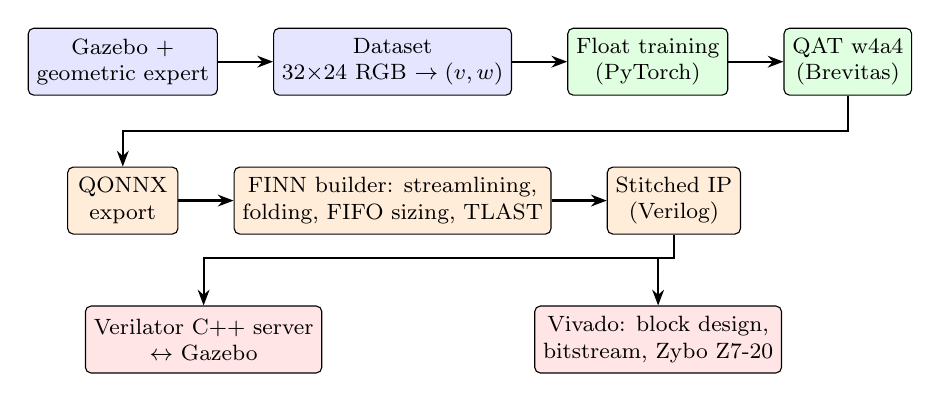
\begin{tikzpicture}[node distance=7mm]
\node[bx=blue!10] (g) {Gazebo +\\geometric expert};
\node[bx=blue!10,right=of g] (d) {Dataset\\$32{\times}24$ RGB $\rightarrow(v,w)$};
\node[bx=green!12,right=of d] (f) {Float training\\(PyTorch)};
\node[bx=green!12,right=of f] (q) {QAT w4a4\\(Brevitas)};
\node[bx=orange!15,below=9mm of g,minimum width=14mm] (o) {QONNX\\export};
\node[bx=orange!15,right=of o] (fb) {FINN builder: streamlining,\\folding, FIFO sizing, TLAST};
\node[bx=orange!15,right=of fb] (ip) {Stitched IP\\(Verilog)};
\node[bx=red!10,below=9mm of fb,xshift=-24mm] (v) {Verilator C++ server\\$\leftrightarrow$ Gazebo};
\node[bx=red!10,below=9mm of ip,xshift=-2mm] (z) {Vivado: block design,\\bitstream, Zybo Z7-20};
\draw[ar] (g)--(d); \draw[ar] (d)--(f); \draw[ar] (f)--(q);
\draw[ar] (q.south) -- ++(0,-4.5mm) -| (o.north);
\draw[ar] (o)--(fb); \draw[ar] (fb)--(ip);
\draw[ar] (ip.south) -- ++(0,-3mm) -| (v.north);
\draw[ar] (ip.south) -- ++(0,-3mm) -| (z.north);
\end{tikzpicture}
\caption{Development flow: from the simulated expert to the hardware. Blue: data; green: training; orange: hardware generation; red: validation in the loop
(simulated RTL and real board).}
\label{fig:flow}
\end{figure}

\subsection{Dataset}
\paragraph{Expert.}
The dataset is generated in Gazebo with a geometric expert that follows the centre line of a circuit (pure pursuit) and chooses its
speed from the curvature, $v(s)=\min(v_{\max},\sqrt{a_{lat}/|\kappa(s)|})$, with limits on acceleration and braking applied forwards and
backwards along the lap ($v_{\max}=12$\,m/s, $a_{lat}=5$\,m/s$^2$). The backward pass makes the expert start braking before a curve, and the forward pass
makes it accelerate only when leaving it, so the speed profile is the one that a careful driver would follow. The centre line and its curvature are extracted automatically
from the mesh of the asphalt of each circuit (skeleton of the road surface, then pushed towards the ridge of maximum clearance), so adding a new circuit only requires its mesh.
The expert uses the true pose of the vehicle; the network only sees the image,
so the speed label is a consistent function of what the camera shows: a straight line far ahead means ``fast'', a line that bends in the lower part of the image means ``brake''.

\paragraph{Recording modes.}
Imitation of a perfect expert is not enough, because the network never sees what happens after its first mistake. Three recording modes are therefore mixed: clean driving;
driving with a temporally correlated perturbation on the angular velocity (the label is the expert's \emph{clean} command, so the network learns to correct the deviation
instead of copying it); and restarts at random
poses 15--30\,m before a curve with lateral offset, heading error and entry speed that can exceed the safe one, which teaches the network to recover and to brake late.
Frames with the vehicle stopped, lateral error above 1.4\,m, or just after a restart are discarded, since their labels do not describe a state that the network
should reproduce.

\paragraph{Image.}
Each camera image is reduced from $640{\times}480$ to $32{\times}24$ RGB (Figure~\ref{fig:camara}); the reduction is the one that the FPGA implements (Section~\ref{sec:flow}),
so training and inference see the same pixels. This detail matters more than it seems: when the reducer in the FPGA averaged whole $30{\times}30$ blocks while training used a
bilinear reduction, the closed loop with the emulated hardware completed only 0.69 of a lap, although the network itself had not changed.

\begin{figure}[t]
\centering
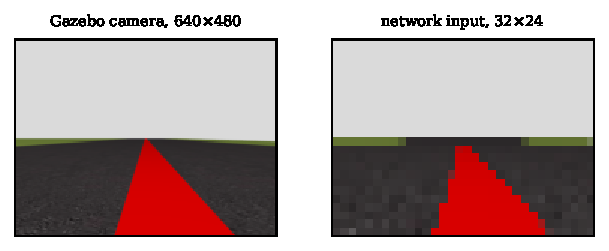
\includegraphics[width=0.75\linewidth]{fig/camara.pdf}\\[2mm]
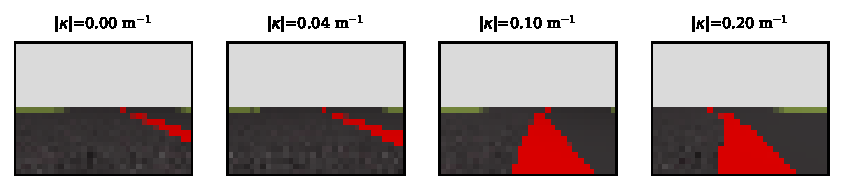
\includegraphics[width=0.95\linewidth]{fig/entradas.pdf}
\caption{Top: a frame of the simulated camera and the $32{\times}24$ image that the network receives. Bottom: four validation inputs of increasing curvature $|\kappa|$ of the
centre line; the red line is the only cue for steering, and the position of the horizon fixes the scale.}
\label{fig:camara}
\end{figure}

\paragraph{Circuits.}
The training set (\texttt{v2} and \texttt{v3}) has 204\,563 frames on three circuits
(Montmel\'o, Montreal, a synthetic circuit) plus 166\,889 frames on two more (a many-curves circuit and Monaco), in both driving directions;
Nürburgring (19\,963 frames) is reserved for validation. Silverstone, built from a public map, is used only for the final closed-loop evaluation (Figure~\ref{fig:circuitos}).
The CNN models (float and quantized), the float MLPs of the \texttt{v3} family and the quantized MLPs \texttt{q4v3} are trained on \texttt{v2}+\texttt{v3}; an earlier
set of quantized MLPs (\texttt{q4}) was obtained from MLPs trained on \texttt{v2} only and is reported separately.
\TODO{table with frames per circuit/mode and the distribution of $v$ and $w$}

\begin{figure}[t]
\centering
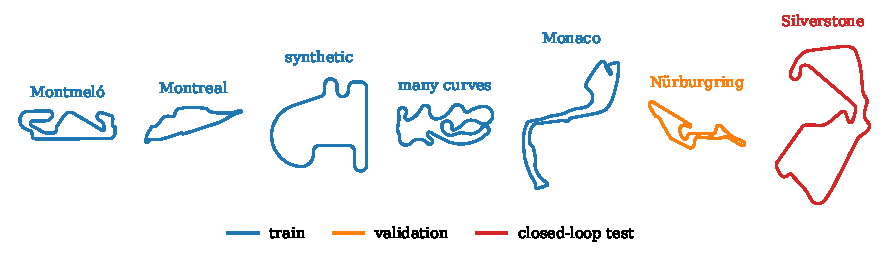
\includegraphics[width=\linewidth]{fig/circuitos.pdf}
\caption{Centre lines of the circuits used for training (blue), validation (orange) and closed-loop test (red). Each circuit is drawn at its own scale.}
\label{fig:circuitos}
\end{figure}

\subsection{Neural model}
Two architectures are compared, both with input $3{\times}24{\times}32$ and two outputs ($v$, $w$, normalized to $[0,1]$ and decoded as
$v\in[-0.6,13]$\,m/s and $w\in[-\pi,\pi]$\,rad/s).
\begin{itemize}
  \item \textbf{MLP}: $2304\rightarrow32\rightarrow256\rightarrow2$ (82\,722 parameters). It treats the image as a vector, so it has no notion of where in the image a pixel is
        except through the weights; it is the cheapest to build, because a fully connected layer maps directly to a matrix-vector engine.
  \item \textbf{Minimal CNN}: two $3{\times}3$ convolutions with stride 2, followed by a dense head (34\,962 parameters). The convolutions share their weights across the image,
        so the network needs fewer parameters and is less sensitive to small shifts of the line.
\end{itemize}
The quantized versions use 4-bit weights and 4-bit activations (w4a4; w4a8 was also explored) and an 8-bit input quantizer. 4-bit products are small enough to be implemented
with look-up tables instead of DSP blocks, which is why none of the generated designs uses any DSP (Section~\ref{sec:flow}).

\subsection{Training}
Both networks are trained on the expert labels with a mean squared error on the normalized outputs, in which curve frames ($|\kappa|\ge0.15$) can be
given a larger weight (curves are a small part of the frames but the part where driving fails), and a one-cycle learning-rate schedule. Floating-point runs use AdamW (weight decay $10^{-4}$); quantization-aware training
with Brevitas starts from the floating-point weights and uses Adam. Script defaults: 40 epochs, learning rate $2\cdot10^{-3}$, batch 1024 (floating point) and
20 epochs, learning rate $3\cdot10^{-4}$, batch 512, curve weight 10 (quantized). Ten random seeds per configuration are trained because
closed-loop performance varies strongly between seeds (Section~\ref{sec:val}): a network with a very good validation error can still fail in one curve.
The floating-point values are the ones recorded in the training logs of the CNN and \texttt{v3} models, with curve weight 10; the quantized runs used 20 epochs with the remaining defaults.
Floating-point training uses the GPU; quantization-aware training runs on the CPU inside the FINN container (about two minutes per MLP model).
\TODO{describe the train/development split (by recording folder)}

\subsection{Inference: from trained model to Verilog implementation}
\label{sec:flow}
\paragraph{Pipeline.} The quantized Brevitas model is exported to QONNX and compiled with FINN v0.9 into a streaming dataflow architecture
(one engine per layer), then stitched into a single IP. The compiler first \emph{streamlines} the graph, absorbing the scale factors and batch-normalization into
integer thresholds so that only integer operations remain; then each layer is mapped to a hardware engine (a matrix-vector unit with PE processing elements and SIMD inputs per element,
and a sliding-window generator for the convolutions); FIFOs between engines are sized by simulation; and the engines are stitched into one block with AXI-Stream
ports. The only FINN limitation we hit for the CNN is that the sliding-window generator
must be the RTL one (the HLS one requires square images). The \emph{folding} (PE and SIMD of each engine) sets the trade-off between resources and cycles; we generate it from a target
number of cycles per image (Table~\ref{tab:fold}).

\paragraph{Camera and reducer.} On the Zybo Z7 the Pcam~5C delivers $1280{\times}720$ RGB through the MIPI CSI-2 receiver, Bayer-to-RGB
conversion and gamma correction. A reducer written in HLS crops the central $4{:}3$ area ($960{\times}720$ columns 160--1119), reduces each $30{\times}30$ block to one pixel
and applies a 256-entry table that implements the 8-bit input quantizer of the network. The reduction is the bilinear one used in training, i.e.\ the mean of the
four central pixels of each block, $(a+b+c+d+2)\gg2$: it needs no division and therefore no DSP, and it matches the reference exactly. Moving the quantizer
to the reducer removes about 3\,k LUT in the CNN and about 31\,k LUT in the MLP, and gives the same integers (checked on 100 real images).
The reducer streams one byte per element, in planar order for the MLP and interleaved RGB pixels for the CNN.

\paragraph{Integration.} Figure~\ref{fig:hw} shows the design. An AXI-Stream switch lets the reduced image go either to a DMA for debugging or to the FINN IP (through a data-width
converter and a clock-domain crossing, since the camera pipeline runs at 150\,MHz and the IP at 100\,MHz); a second DMA collects the network output (two signed 16-bit words, the integer values of $v$ and $w$)
and the ARM applies the final scale and offset. The camera interface is a unmodified Digilent design; the HDMI output used for debugging was removed to free logic.
For the validation with the simulator the camera is replaced by a third DMA that reads a $1280{\times}720$ frame from the DDR memory (dashed in the figure), so the same
reducer and the same IP process the frames of Gazebo (a second switch selects between the camera and this DMA).

\begin{figure}[t]
\centering
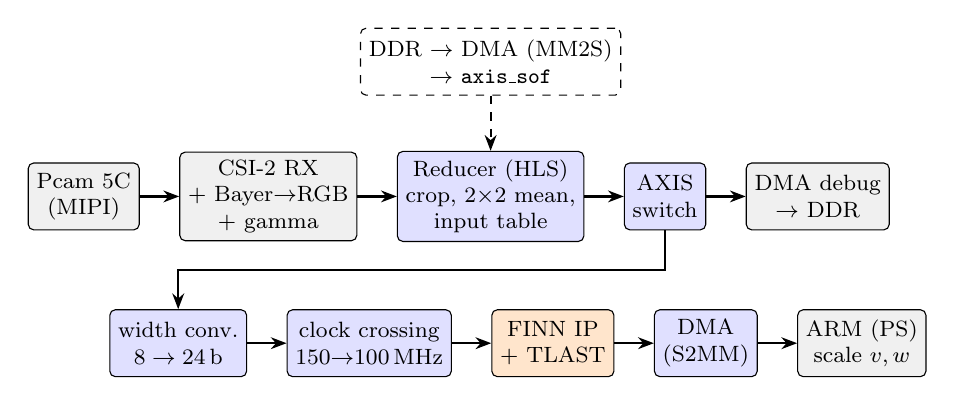
\begin{tikzpicture}[node distance=5mm]
\node[bx=gray!12] (cam) {Pcam 5C\\(MIPI)};
\node[bx=gray!12,right=of cam] (rx) {CSI-2 RX\\+ Bayer$\rightarrow$RGB\\+ gamma};
\node[bx=blue!12,right=of rx] (red) {Reducer (HLS)\\crop, $2{\times}2$ mean,\\input table};
\node[bx=blue!12,right=of red] (sw) {AXIS\\switch};
\node[bx=white,above=7mm of red,dashed] (hil) {DDR $\rightarrow$ DMA (MM2S)\\$\rightarrow$ \texttt{axis\_sof}};
\node[bx=blue!12,below=10mm of cam,xshift=12mm] (dw) {width conv.\\$8\rightarrow24$\,b};
\node[bx=blue!12,right=of dw] (cdc) {clock crossing\\150$\rightarrow$100\,MHz};
\node[bx=orange!20,right=of cdc] (fin) {FINN IP\\+ TLAST};
\node[bx=blue!12,right=of fin] (d1) {DMA\\(S2MM)};
\node[bx=gray!12,right=of d1] (ps) {ARM (PS)\\scale $v,w$};
\node[bx=gray!12,right=of sw] (d0) {DMA debug\\$\rightarrow$ DDR};
\draw[ar] (cam)--(rx); \draw[ar] (rx)--(red); \draw[ar] (red)--(sw);
\draw[dr] (hil)--(red);
\draw[ar] (sw.south) -- ++(0,-5mm) -| (dw.north);
\draw[ar] (sw)--(d0);
\draw[ar] (dw)--(cdc); \draw[ar] (cdc)--(fin); \draw[ar] (fin)--(d1); \draw[ar] (d1)--(ps);
\end{tikzpicture}
\caption{Hardware design on the Zybo Z7-20. The solid path is the camera path; the dashed block replaces the camera in the hardware-in-the-loop design.
The FINN IP generates its own TLAST, so the output DMA closes each packet of two 16-bit words.}
\label{fig:hw}
\end{figure}

\paragraph{Packet boundary.} The IP stitched by FINN has no TLAST signal on its output stream, so the output DMA never saw the end of the packet and flagged an
internal error even though the four bytes of the result were correct. We first solved it with a few lines of Verilog, and then replaced them with the \emph{TLastMarker}
that the FINN builder provides: a node inserted after the FIFOs, with its own HLS IP, that raises TLAST on the second output word (+50 LUT). Every IP of this work
(MLP and the three CNN variants) is now generated by FINN alone, with no hand-written logic in the data path, and on the real board the DMA reports no error.

\paragraph{Bit-exactness.} Four checks, all against the Brevitas model: (i) rtlsim of the stitched IP in FINN on real images,
(ii) rtlsim on 60 images that the quantized model saw while driving in Gazebo (max.\ difference $<3\cdot10^{-6}$ in $v$ and $w$),
(iii) a native C++/Verilator simulation of the generated Verilog with the same packing of the input stream as the hardware (30 images,
max.\ difference $2.9\cdot10^{-6}$), and (iv) the reducer in HLS C simulation and in RTL simulation, bit-exact with the golden model.
On the board, the reduced image is identical to the reference in every pixel and $v$, $w$ equal those of the Verilator simulation.
A detail worth reporting: FINN packs each input element with the number of bits of its data type, so a 7-bit input annotation does not match
a byte-oriented stream; the input is annotated as 8 bit. This kind of error is invisible to the offline check of the network and appears as soon as the real stream is connected.

\paragraph{Resources and latency.}
Table~\ref{tab:res} gives the cost of the whole design (camera path, reducer and FINN IP, no HDMI) on the Zybo Z7-20; Table~\ref{tab:fold} isolates the FINN IP and shows
what the folding buys.
\begin{table}[h]
\centering
\caption{Integrated design on the Zybo Z7-20 (Vivado 2022.2, camera path + reducer + FINN IP, no HDMI).
Final builds with the input annotated as 8 bit. The MLP does not fit in the Z7-10 (94\% LUT).}
\label{tab:res}
\begin{tabular}{lrrrr}
\toprule
 & LUT & FF & BRAM tiles & Power (W)\\
\midrule
CNN w4a4 (min.\ folding) & 13\,687 (25.7\%) & 17\,864 & 34.5 & 2.02\\
MLP w4a4 (min.\ folding) & 16\,659 (31.3\%) & 31\,600 & 39 & 2.09\\
\bottomrule
\end{tabular}
\end{table}
With the IP generating TLAST the camera design with the CNN folded by 8 uses 14\,760 LUT, the MLP 16\,639 and the hardware-in-the-loop design 16\,049; there are no DSP blocks in any of them. Rebuilt with TLAST, the original CNN needs 13\,670 LUT and 34.5 BRAM tiles (2.02\,W) and the fully parallel one 15\,699 LUT and 30 BRAM tiles (2.06\,W), so in the complete design the extra parallelism costs about 15\,\% more LUT.
Timing closes everywhere except on the MIPI input pins, where the constraint is not met (worst slack $-2.45$\,ns) in all variants, as in the earlier builds of this design.

\begin{table}[h]
\centering
\caption{FINN IP of the CNN for three levels of parallelism, synthesized out of context for the Z7-20 at 100\,MHz (with TLAST).
Cycles are those of the RTL simulation; the three IPs give exactly the same output on six random images.}
\label{tab:fold}
\begin{tabular}{lrrrrrr}
\toprule
IP & Cycles & Latency (ms) & LUT & BRAM18/36 & DSP & WNS (ns)\\
\midrule
Original (PE=SIMD=1) & 91\,425 & 0.91 & 5\,713 & 23 / 9 & 0 & $+1.20$\\
Folded $\times8$ & 10\,716 & 0.11 & 6\,730 & 21 / 8 & 0 & $+0.98$\\
Parallel ($T{=}1800$) & 4\,729 & 0.047 & 7\,946 & 22 / 6 & 0 & $+0.74$\\
\bottomrule
\end{tabular}
\end{table}
At 100\,MHz the FINN IP needs 91\,400 clock cycles (0.91\,ms) per image for the CNN and 26\,900 (0.27\,ms) for the MLP at minimum folding (PE=SIMD=1);
this is far below the 50--100\,ms control period, and an MLP IP costs 8\,503 LUT out of context. Increasing the parallelism by 20 times reduces the cycles by the same factor
(Figure~\ref{fig:fold}) for 39\,\% more LUT, because most of the logic of the CNN is not in the arithmetic: the weights live in the block RAM and the sliding-window generator
does not get cheaper when the engines get wider. The floor of about 1\,800 cycles for the CNN is set by that generator, which processes at most three channels per cycle.
The analytical estimate of FINN overestimates the parallel design (14\,600 LUT against 7\,900 after synthesis), so the estimate should be used to rank folding options but not to
decide whether a design fits. The MLP does not fit in the Z7-10; the CNN fits but misses timing at 150\,MHz inside the
Xilinx VDMA used for full-frame capture.

\begin{figure}[t]
\centering
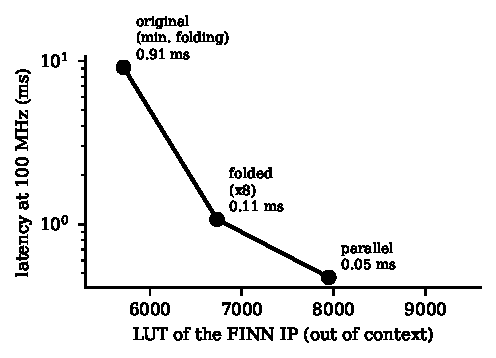
\includegraphics[width=0.65\linewidth]{fig/plegado.pdf}
\caption{Latency against logic for the three CNN IPs of Table~\ref{tab:fold}: a 20-fold reduction in latency costs 39\,\% more LUT and no DSP.}
\label{fig:fold}
\end{figure}

\section{Experimental validation}
\label{sec:val}

\subsection{Visual follow line application}
The robot is a $0.99{\times}0.36$\,m holonomic vehicle controlled with \texttt{/cmd\_vel}; the network chooses $v$ and $w$ from the image of a red centre line
on dark asphalt, 20\,Hz camera. A run is successful if the vehicle completes the laps without being stuck; we also record the maximum lateral error with respect to the centre line.
All closed-loop evaluations start the vehicle on the start line of the circuit and are run in both driving directions; a vehicle is considered stuck when it stops advancing.
Each cell of the following tables is a single run, and the simulator is not deterministic, so differences of a few runs between two configurations are within the noise.

\subsection{FPGA-Robotics with Gazebo simulator}
\paragraph{Networks in closed loop.}
On Silverstone (never seen in training), 2 laps in both directions with 10 seeds per model (20 runs), Table~\ref{tab:sil} shows that both networks work and that the CNN is the more robust one;
the 4-bit quantization costs it nothing in this test.
\begin{table}[h]
\centering
\caption{Closed-loop success on Silverstone (2 laps, both directions, 10 seeds).}
\label{tab:sil}
\begin{tabular}{lcc}
\toprule
Model & Success & Rate\\
\midrule
CNN float & 17/20 & 85\%\\
CNN w4a4 & 17/20 & 85\%\\
MLP w4a4 & 14/20 & 70\%\\
MLP float & 12/20 & 60\%\\
\bottomrule
\end{tabular}
\end{table}
Part of the failures happen in one curve independent of the track width.

A fairer comparison of the quantized networks uses the same training data, the same number of epochs and the same quantization for both. Table~\ref{tab:mc} and Figure~\ref{fig:lc} give the
two-lap completions on Montmel\'o and Nürburgring, in both directions with 10 seeds (40 runs per model). The MLP retrained on \texttt{v2}+\texttt{v3} (\texttt{q4v3}) improves a little over the one
trained on \texttt{v2} only (13 to 17 of 40, mostly on Nürburgring), but the CNN completes twice as many runs (34 of 40) with the same data. The advantage of the CNN is therefore not due to having been
trained with more data. The MLP depends much more on the seed: some seeds complete three of four runs and others none, while the CNN is stable.
\begin{table}[h]
\centering
\caption{Two-lap completions of the quantized (w4a4) networks, 10 seeds $\times$ 2 directions per circuit. \texttt{q4}: MLP from floating-point weights trained on \texttt{v2} only;
\texttt{q4v3}: MLP trained on \texttt{v2}+\texttt{v3}; \texttt{cq4}: CNN, \texttt{v2}+\texttt{v3}.}
\label{tab:mc}
\begin{tabular}{lcccc}
\toprule
Model & Montmel\'o & Nürburgring & Total & Mean laps (M / N)\\
\midrule
MLP \texttt{q4} & 8/20 & 5/20 & 13/40 & 1.26 / 1.05\\
MLP \texttt{q4v3} & 6/20 & 11/20 & 17/40 & 1.24 / 1.35\\
CNN \texttt{cq4} & 15/20 & 19/20 & 34/40 & 1.76 / 2.00\\
\bottomrule
\end{tabular}
\end{table}
\begin{figure}[t]
\centering
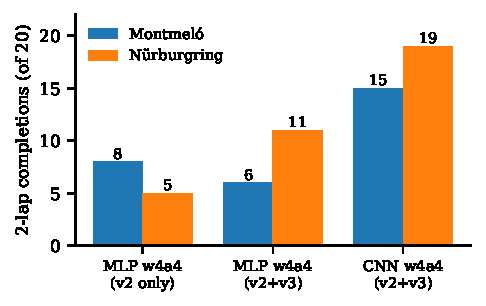
\includegraphics[width=0.6\linewidth]{fig/lazo_cerrado.pdf}
\caption{Two-lap completions out of 20 runs per circuit for the three quantized models of Table~\ref{tab:mc}.}
\label{fig:lc}
\end{figure}
\TODO{confidence intervals or repetitions per cell; table per seed}

\paragraph{Track width.}
Narrowing the track while keeping the centre line shows that the networks need a semi-width of roughly 0.8--1.0\,m (4.5--5.5 times the vehicle width)
in this simulator: 0 or 1 of 6 runs succeed at 0.8\,m and 4--5 of 6 at 1.0\,m. This is a property of the simulated vehicle and not a claim for real robots.

\paragraph{Loop rate and delay.}
A hardware implementation adds latency (camera, reducer, network, communication) and may run at a lower rate than the simulator, so we measured how much of both the controller tolerates.
\begin{table}[h]
\centering
\caption{Quantized models in closed loop under a slower control rate and a delay in the command (1 lap, Silverstone, speed scaled by 0.25).}
\begin{tabular}{lcc}
\toprule
Condition & CNN w4a4 & MLP w4a4\\
\midrule
20\,Hz, no delay & 2/2 & 2/2\\
20\,Hz, 50\,ms & 2/2 & 2/2\\
10\,Hz, 50\,ms & 2/2 & 2/2\\
5\,Hz, 100\,ms & 2/2 & 2/2\\
\bottomrule
\end{tabular}
\end{table}
At full speed (8.7\,m/s) every condition with a delay failed (0/2 for both models), since 50\,ms are 0.44\,m of travel; the slow-motion scale
(2.2\,m/s) mimics a real robot, whose speeds are about an order of magnitude lower. \TODO{note on the scale; the full-speed table}

\paragraph{FPGA in the loop (Verilator).}
The generated Verilog of the CNN is simulated with Verilator in a C++ UDP server (Figure~\ref{fig:fil}, left path): Gazebo sends each $32{\times}24$ image, the server applies the reducer
table, feeds the AXI-Stream input, collects the two output words and returns $v$ and $w$. Because Verilator is slower than real time, Gazebo is paused while the IP answers and the delay of the
hardware chain is added explicitly (50\,ms), so that the simulated robot sees the same delay as with the real hardware but the experiment does not depend on how fast the host is.
The simulation time per image depends directly on the cycles of the IP: 0.108\,s for the original CNN, 0.009\,s for the folded one and 0.004\,s for the parallel one (0.019\,s for the MLP).

\begin{figure}[t]
\centering
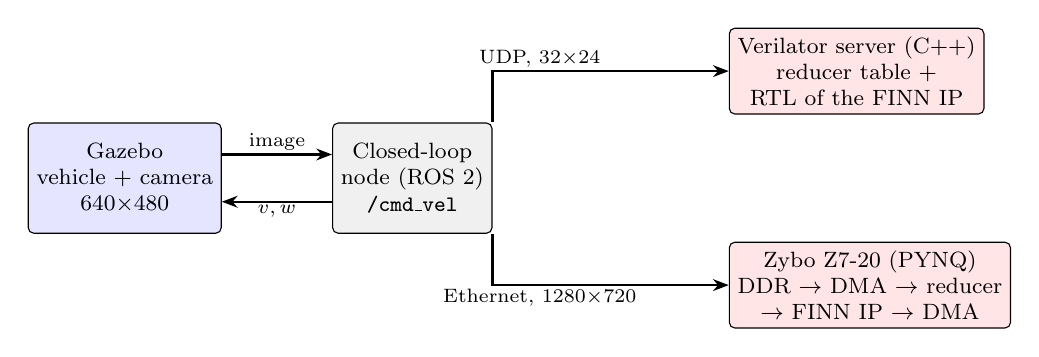
\begin{tikzpicture}[node distance=9mm]
\node[bx=blue!10,minimum height=14mm] (gz) {Gazebo\\vehicle + camera\\$640{\times}480$};
\node[bx=gray!12,right=14mm of gz,minimum height=14mm] (ctl) {Closed-loop\\node (ROS 2)\\\texttt{/cmd\_vel}};
\node[bx=red!10,above right=1mm and 30mm of ctl] (vs) {Verilator server (C++)\\reducer table +\\RTL of the FINN IP};
\node[bx=red!10,below right=1mm and 30mm of ctl] (zy) {Zybo Z7-20 (PYNQ)\\DDR $\rightarrow$ DMA $\rightarrow$ reducer\\$\rightarrow$ FINN IP $\rightarrow$ DMA};
\draw[ar] ([yshift=3mm]gz.east) -- node[lb,above] {image} ([yshift=3mm]ctl.west);
\draw[ar] ([yshift=-3mm]ctl.west) -- node[lb,below] {$v,w$} ([yshift=-3mm]gz.east);
\draw[ar] (ctl.north east) |- node[lb,pos=.6,above] {UDP, $32{\times}24$} (vs.west);
\draw[ar] (ctl.south east) |- node[lb,pos=.6,below] {Ethernet, $1280{\times}720$} (zy.west);
\end{tikzpicture}
\caption{FPGA in the loop. Left path: the RTL of the IP simulated with Verilator on the host, with Gazebo paused during each inference. Right path: the IP implemented on the real board,
which receives the frame over Ethernet and returns $v$ and $w$.}
\label{fig:fil}
\end{figure}

\paragraph{System timing.}
Table~\ref{tab:sys} gives the one-lap time of Silverstone for the three CNN IPs, with Gazebo paused (speed scale 0.5, 5\,Hz). Folding the IP reduces the wall-clock time of a lap by 23\,\%
(288\,s to 223\,s) because the IP simulation stops being the dominant cost; after that the simulator itself (Gazebo and ROS) takes most of the time and the parallel IP is not faster (222\,s).
The three IPs give the same output for the same image, so the differences in maximum lateral error between runs (0.42--0.81\,m) come from the variability of the simulator
and not from the network (we did not measure its dispersion). Running without pausing the simulator, at the full speed scale (1.0) and 10\,Hz, none of the three completes the lap
(0.15, 0.71 and 0.13 of a lap): at that speed the limit is the controller, not the speed of the IP.
\begin{table}[h]
\centering
\caption{Closed loop with the Verilator IP on Silverstone, one lap, one run per row.}
\label{tab:sys}
\begin{tabular}{lcccc}
\toprule
Mode / IP & Verilator per image & Simulated time & Wall-clock time & Max.\ lateral error\\
\midrule
0.5$\times$, 5\,Hz, paused: original & 0.114\,s & 157.7\,s & 288\,s & 0.71\,m\\
0.5$\times$, 5\,Hz, paused: folded & 0.010\,s & 158.0\,s & 223\,s & 0.42\,m\\
0.5$\times$, 5\,Hz, paused: parallel & 0.004\,s & 158.8\,s & 222\,s & 0.81\,m\\
\bottomrule
\end{tabular}
\end{table}

\paragraph{Hardware in the loop with the real board.}
In the last stage the IP is not simulated: Gazebo's image is enlarged and centred in a $1280{\times}720$ frame with black bands (the format of the camera), published as a ROS~2 message,
sent over Ethernet to the Zybo Z7-20 running PYNQ, stored in the DDR memory and streamed by DMA through the same reducer and FINN IP as in the camera design;
the board returns the command as a message to the simulator (right path of Figure~\ref{fig:fil}). In a test without ROS the reduced image is identical to the reference in every pixel and the
result equals that of the Verilator simulation; the board needs 18.6\,ms per frame, dominated by the transfer. With the same conditions as the Verilator runs (speed scale 0.5, 5\,Hz, paused),
the closed loop with the board completes one lap of Silverstone with a maximum lateral error of 0.45\,m (Figure~\ref{fig:tray}).
The first runs showed a latency of the server with isolated peaks of 8\,s. Their origin was the start-up order: the first ten queries of the loop were sent before the bridge to the board
existed and waited for the 8\,s connection retry. Starting the bridge before the loop removes them; in all the runs below the latency has no peaks.

\paragraph{Statistics with the board.}
To measure the dispersion we repeat the experiment with three seeds, two circuits (Silverstone, Montmel\'o) and both directions of travel, for each of the three CNN IPs loaded in the board
(12 laps per IP, 36 in total). Each seed perturbs the start pose of the robot with a lateral offset in $[-0.4,0.4]$\,m and a heading offset in $[-0.12,0.12]$\,rad. All 36 laps are completed
(1.0 laps, no errors, no stalls). Table~\ref{tab:hil} gives the maximum lateral error and the latency of the server (query sent from the simulator until the command is received).
The three IPs are indistinguishable within the dispersion between seeds: the global maximum error is 0.41\,m (folded and original) and 0.45\,m (parallel),
the latter due mostly to one lap of Silverstone with 0.73\,m that was completed. The hardest case for every IP is Silverstone in the reverse direction (0.52--0.61\,m).
The latency is $0.345$--$0.360$\,s on average with a 95th percentile of at most 0.384\,s and a maximum of 0.487\,s; the 18.6\,ms of the board are a small part of it, the rest is
the transport of the $1280{\times}720$ frame and the ROS~2 and TCP bridge.
\begin{table}[h]
\centering
\caption{Closed loop with the IP on the Zybo Z7-20: maximum lateral error (m), mean $\pm$ standard deviation over three seeds (one lap each).}
\label{tab:hil}
\begin{tabular}{llccc}
\toprule
Circuit & Direction & Folded & Original & Parallel\\
\midrule
Silverstone & $+1$ & $0.43\pm0.04$ & $0.37\pm0.06$ & $0.50\pm0.21$\\
Silverstone & $-1$ & $0.52\pm0.06$ & $0.61\pm0.03$ & $0.54\pm0.07$\\
Montmel\'o & $+1$ & $0.37\pm0.04$ & $0.35\pm0.02$ & $0.37\pm0.02$\\
Montmel\'o & $-1$ & $0.33\pm0.06$ & $0.33\pm0.06$ & $0.38\pm0.03$\\
\midrule
All (12 laps) & & $0.41\pm0.09$ & $0.41\pm0.12$ & $0.45\pm0.12$\\
Server latency, mean (s) & & 0.360 & 0.345 & 0.345\\
Server latency, max.\ 95th pct.\ (s) & & 0.384 & 0.367 & 0.368\\
\bottomrule
\end{tabular}
\end{table}

\begin{figure}[t]
\centering
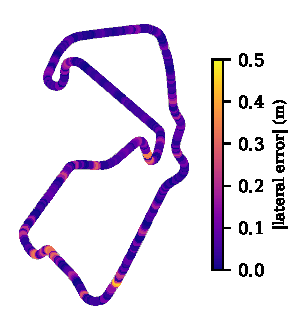
\includegraphics[width=0.55\linewidth]{fig/trayectoria_placa.pdf}
\caption{Lap of Silverstone driven by the CNN running on the Zybo Z7-20 inside the simulation loop, coloured by the absolute lateral error (maximum 0.45\,m).}
\label{fig:tray}
\end{figure}

\paragraph{What the loop catches.}
Two of the errors found in this work are invisible to an offline test and were only found when the hardware drove the robot: the input annotated with 7 bits that did not match
the byte-oriented stream, and the reducer that averaged blocks instead of using the bilinear reduction of the training. In both cases the network was correct and the numbers were wrong
by a small amount, and only the closed loop showed that it was enough to leave the lane.

\subsection{Physical Robot}
\TODO{not done. Plan: a TurtleBot-like robot following a red line (3M 764 vinyl tape, 50\,mm, for a Burger; 100--120\,mm for larger robots) on a dark matte floor without borders;
Zybo Z7-20 + Pcam~5C; speeds rescaled as $v_{real}=s\,\tau\,v_{sim}$, $w_{real}=\tau\,w_{sim}$ with $\tau\approx0.06$; main risk: the real camera is higher or tilted compared with the simulated one,
which may require retraining with the real geometry.}

\section{Conclusions}
\label{sec:concl}
We have presented a flow that goes from a simulated expert to a quantized network on a low-cost FPGA and that is validated, at each stage, with the robot in the loop.
Four conclusions can be drawn from the results.
First, the flow is reproducible and ends in the same simulator where it started: the dataset, the quantized network, the RTL of the IP and the real board drive the same robot on the same circuits.
Second, in closed loop the CNN is more robust than the MLP with the same data (34 against 17 completions out of 40), even though the MLP is cheaper in cycles (26\,900 against 91\,400 at minimum folding);
the quantization to 4 bits costs the CNN nothing on Silverstone (17 of 20 in both cases).
Third, the folding of the CNN reduces its latency by a factor of 20 (0.91 to 0.047\,ms) for 39\,\% more LUT and no DSP, but the control period (50--100\,ms) is far larger than any of these latencies, so
at this scale parallelism is a margin and not a requirement; the gain is in the time needed to simulate the system.
Fourth, the closed loop with the hardware finds integration errors that the offline checks miss.
The limits are as important as the results: each cell of the simulated tables is a single run, the board has been tested with three seeds per cell but always with the image of the simulator, not with the real camera, and the physical robot is still to be done.
\TODO{physical robot; next steps: real camera in the loop, real-time simulation}

\begin{thebibliography}{9}
% TODO: check every entry (authors, year, venue, pages) before submission.
\bibitem{koenig2004gazebo} N.~Koenig and A.~Howard, ``Design and use paradigms for Gazebo, an open-source multi-robot simulator,'' in \emph{IEEE/RSJ IROS}, 2004.
\bibitem{macenski2022ros2} S.~Macenski, T.~Foote, B.~Gerkey, C.~Lalancette, and W.~Woodall, ``Robot Operating System 2: Design, architecture, and uses in the wild,'' \emph{Science Robotics}, vol.~7, no.~66, 2022.
\bibitem{bojarski2016end} M.~Bojarski \emph{et al.}, ``End to end learning for self-driving cars,'' arXiv:1604.07316, 2016.
\bibitem{umuroglu2017finn} Y.~Umuroglu \emph{et al.}, ``FINN: A framework for fast, scalable binarized neural network inference,'' in \emph{ACM/SIGDA FPGA}, 2017.
\bibitem{brevitas} A.~Pappalardo, ``Brevitas: neural network quantization in PyTorch,'' software, Xilinx/AMD.
\bibitem{duarte2018hls4ml} J.~Duarte \emph{et al.}, ``Fast inference of deep neural networks in FPGAs for particle physics,'' \emph{Journal of Instrumentation}, vol.~13, 2018.
\bibitem{jacob2018quantization} B.~Jacob \emph{et al.}, ``Quantization and training of neural networks for efficient integer-arithmetic-only inference,'' in \emph{IEEE/CVF CVPR}, 2018.
\end{thebibliography}

\end{document}
